\sectionmark{Stoffkreisläufe}

\section{Stoffkreisläufe}

\begin{figure}
	\leavevmode
	\begin{center}
	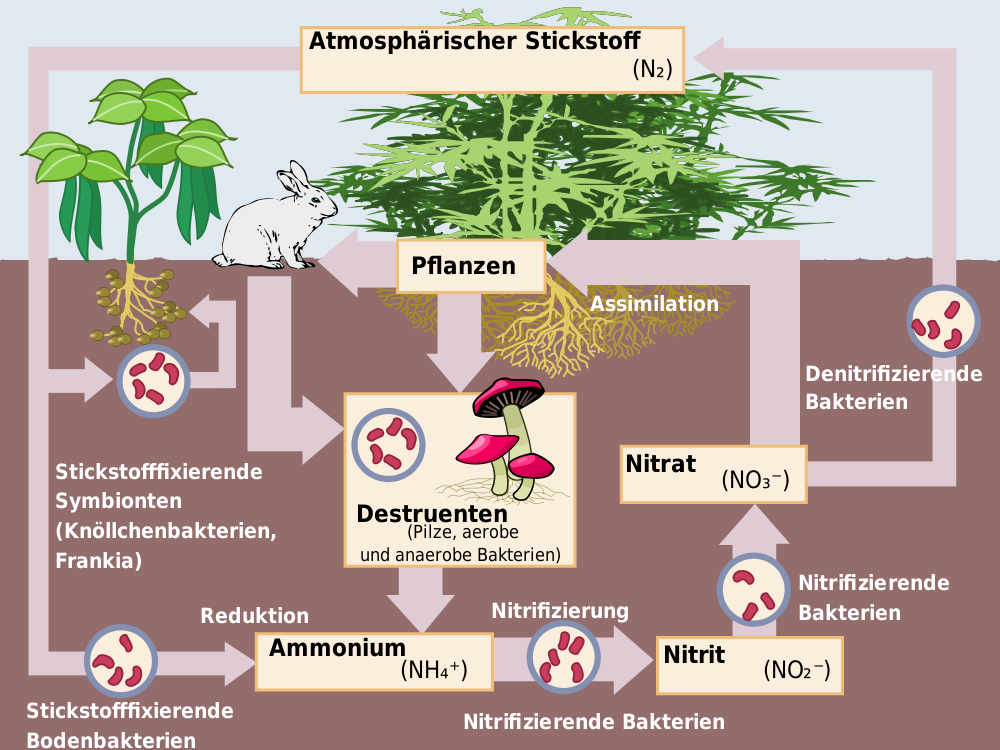
\includegraphics[scale=0.33]{./pictures/stickstoff_kl_1000}
	\end{center}
	\caption{\slshape{Der Stickstoffkreislauf.}}
	\label{fig:Duennfluessigkeitweggehen}
	%http://de.wikipedia.org/wiki/Datei:Cicle_del_nitrogen_de.svg
\end{figure}

\begin{enumerate}
	\item Nennen sie dissimilatorische Prozesse im Stickstoff-Kreislauf?
		
		\begin{itemize}
			\item Anaerobe Denitrifikation \hfill \ce{NO3-} \textrightarrow \ce{NO2-} \textrightarrow \ce{N2}
			\item Aerobe Denitrifikation \hfill \ce{NO4+} \textrightarrow \ce{NO2-} \textrightarrow \ce{NO3-}
			\item Anammox \hfill \ce{NO2-},\ce{NH4+} \textrightarrow \ce{N2}
			\item Assimilation \hfill \ce{NH4+} \textrightarrow \ce{NH3}
		\end{itemize}

		Eine Übersich über den Stickstoffkreislauf findet sich in Abbildung \ref{fig:Duennfluessigkeitweggehen} auf Seite \pageref{fig:Duennfluessigkeitweggehen}.


	\item Welche Rolle spielen Denitrifikanten und Nitrifikanten bei der Abwasserbehandlung in Kläranlagen?

		Durch Denitrifikation geschieht die Stickstoff-Eleminierung.
		Dies kann auch durch das Anammox-Verfahren geschehen,
		bei dem jedoch weniger Biomasse endsteht.

		Bei der Denitrifikation wir zunächst aerob \ce{NH4+} in \ce{N03-} unter \ce{O2}-Gabe umgesetzt.
		Dann wird das \ce{NO3-} mit organimschem Kohlenstoff,
		beispielsweise aus Methanol,
		in Stickstoffgas und Biomase umgesetzt.

		Beim Aanmmox-Verfharen wird  die Hälfte des \ce{NH4+} mit \ce{O2} in\ce{NO2-} umgestetzt.
		Dieses wird zusammen mit dem restlichen \ce{NH4+} in Stickstoffgas und wenig Biomase umgesetzt.

	\item Welche Umsetzung katalysieren Anammox-Bakterien?

		Anammox Bakterien katalysieren die Umsetzung von Ammonium und Nitrit zu Stickstoffgas und Wasser.\\
		\begin{center}
			\ce{NH4+} + \ce{N02-} \textrightarrow \ \ce{N2} + 2 \ce{H2O} 
		\end{center}

	\item Nennen Sie \ce{N2}-Fixierer!
	
		\begin{itemize}
			\item Rhizobien in Symbiose mit Leguminosen
			\item Phototrophe Bakterien 
				\begin{itemize}
					\item Cyanobakterien 	\hfill (oxygene Photosynthese)
					\item Purpurbakterien 	\hfill (anoxygene Photosynthese)
					\item Grüne Bakterien 	\hfill (anoxygene Photosynthese)
				\end{itemize}
			\item Azotobacter vinelandii 	\hfill(Aerobier)
			\item einige Clostriedien		\hfill(Anaerobier)
		\end{itemize}

	\item Können eukaryontische Organismen \ce{N2} fixieren?
		
		Nein, nur die ``Bacteria'' sind in der lage molekularen Stickstoff zufixieren.

	\item Wie ist Nitrogenase aufgebaut?
		
		Die Nitrogenase ist ein Enzymkomplex der mehrere Redox-Zentren besitzt.
		Schlüsselkomponentenen sind dabei die Nitrogenase-reductase und die Nitrogenase.
		Wobei der Elektronentransfer von der Reductase zur Nitrogenase nur unter ATP verbauch möglich ist.

		\begin{description}
			\item[Nitrogenase Reductase] \hfill \\
				\begin{itemize}
					\item Dimer aus zwei identischen Untereinheiten
					\item enthält eine einzelnes 4\ce{Fe}-4\ce{s} Redox-zentrum
					\item stellt Elektronen mit großem Reduktionspotential bereit.
				\end{itemize}
			\item[Nitrogenase] \hfill \\
				\begin{itemize}
					\item Tetramer, 2 mal 2 identische Untereinheiten
					\item Ein Redox-Zentrum pro Tetramer mit 2 \ce{Mo}, 32 \ce{Fe} und 30 \ce{S}
					\item benutz \ce{e-} um \ce{N2} zu \ce{NH3} zu reduzieren
					\item \slshape{hochgradig empfindlich gegenüber Sauerstoff}
				\end{itemize}
		\end{description}

	\item Beschreiben Sie den Ablauf der \ce{N2}-Reduktion an der Nitrogenase!

		\begin{center}
			\ce{N2} + 10\ce{H+} + 8\ce{e-} + 16ATP \textrightarrow \ 2\ce{NH4+} + 16ADP + 16P\textsubscript{i} + \ce{H2}
		\end{center}

	\item Wie kann die Nitrogenase vor dem Kontakt mit Sauerstoff geschützt werden?

		Der Schutz der Nitrogenase kann auf vielfältige Weise geschehen.
		So erfolgt der Schutz durch Kapselung oder Schleimschichten.
		Bakterien die oxygene Photosynthese betreiben,
		habe die Stickstofffixierung in sogenannte Heterocysten ausgelagert,
		welche sich auf diesen Vorgang spezialisiert haben.
		Auch gibt es Bakterien die die Stickstofffixierung nur nachts durchführen,
		wenn die Lichtreaktion der Photosynthese ruht.
		So erfolgt eine zeitliche Trennung.

	\item Welche Rolle spielen phototrophe Bakterien im Schwefel-Kreislauf?

		Sie können \ce{SO42-} in \ce{H2S} Umsetzen.
		Dies geschieht durch \ce{S0}-Respiration.

	\item An welchen Schritten im Stickstoff- und Schwefel-Kreislauf sind chemolithoautotrophe Organismen beteiligt (Nennen sie Namen für typische Vertreter)?
		\label{item:gebaeudefresser}

		\begin{description}
			\item[Schwefel] \hfill \\
				\begin{itemize}
					\item \emph{Thiobacillus thiooxidans} \hfill \ce{H2S} + 2 \ce{O2} \textrightarrow \ \ce{H2SO4}
					\item Gattung \emph{Desulfovibrio} \hfill 4\ce{H2} + \ce{H2SO4} \textrightarrow \ \ce{H2S} + 4 \ce{H2O}
				\end{itemize}
		\end{description}

	\item Welche Organismengruppen können für Gebäudeschäden verantwortlich sein und warum?
		
		Organismen die als Stoffwechselprodukt \ce{H2S} haben,
		da diese mit Wasser zu Schweliger- bzw. Schwefelsäure werden kann.
		Diese kann beispielsweise Gebäude aus Sandstein angreifen.
		Siehe dazu auch die Aufstellung aus Frage \ref{item:gebaeudefresser}.

	\item Welche Rolle spielen Sulfatreduzierer im Schwefel-Kreislauf?

		Sie sorgen für die Schwefelwasserstoff zu molekularem Schwefel oder Sulfat umgesetzt.

\end{enumerate}
